\chapter{Introduction}
\label{sec:introduction-chapter}

\section{The Capacitated Vehicle Routing Problem}
\label{sec:intro-cvrp-problem}

The Capacitated Vehicle Routing Problem (\textbf{CVRP}), first presented in \textcite{dantzig1959}
under the name of "truck dispatching problem",
is one of the most studied combinatorial optimization routing problem.
The CVRP is an NP-hard (in the strong sense) problem which can be considered a generalization
of the well-known Travelling Salesman Problem (TSP).
The TSP \parencite{flood1956}
is an NP-hard \parencite{garey1976planar} ubiquitous combinatorial optimization problem in the operations research field,
that asks for the determination of a Hamiltonian circuit of minimum cost
\parencite{croes1958, laporte1992,johnson1997,applegate2006,gutin2006,hoffman2013}.
The CVRP can be defined verbally as finding an optimal route for a transportation/distribution/delivery problem
starting from a common point called the depot,
where a homogeneous fleet composed of a fixed number of trucks, subject to capacity constraints,
need to serve customer demands of a single good (i.e. delivery of gasoline to gas stations).
Given as input: a weighted graph representing the road network,
the customer demands and the vehicle capacity,
the problem consists in determining a set of routes, one for each vehicle,
of minimal overall travel distance starting and ending at the depot.
The set of routes need to serve all the customers in the road network exactly once and no more
\parencite{toth2014}.
A diagram showing an example of a CVRP problem along with one of its feasible solution
is provided in \Cref{fig:cvrp-optimal-solution-example}.

\begin{figure}[ht]
	\centering
	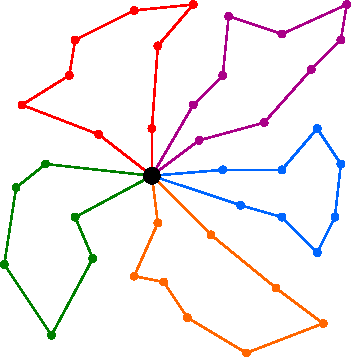
\includegraphics[width=12cm]{Imgs/P-n40-k5-solution.out.cropped.pdf}
	\caption{An example of a feasible solution to a CVRP problem (instance named P-n40-k5).
		There are 39 customers to be served and 5 available trucks with capacity $140$ each. Each color
		represents a different route taken by each truck and the colored dots
		represents the customers served on each route.
		The larger black dot represents the central facility (the depot).
		Credits: \url{http://vrp.galgos.inf.puc-rio.br/index.php/en/plotted-instances?data=P-n40-k5}.
	}
	\label{fig:cvrp-optimal-solution-example}
\end{figure}

Studying effective solution methods for the CVRP may lead to tremendous real-world economic
savings for the management of the provision of goods or services in a distribution system.
Optimal delivery planning can reduce the overall transportation and good costs while
also reducing the waiting time experienced by the customers.
Therefore, studying optimal efficient algorithms and mathematical models for
solving and describing real-world distribution problems,
becomes of vital importance
for the operational management of a cost-efficient planning process \parencite{toth2002,toth2014}.

The CVRP belongs to the wider class of problems known as the Vehicle Routing Problems (VRPs).
There are many variations of VRPs proposed in the literature such as
the Vehicle Routing Problem with Time Windows (VRPTW), and many others.
In the VRPTW \parencite{schrage1981} the vehicles are subject to capacity constraints and
each customer is associated with a time window slot in which it can be served,
Nonetheless, CVRP is the simpler VRP variant to describe,
and yet to this day, it remains the most central and studied routing problem.
For a more complete taxonomy on the many VRP variants refer to \textcite{eksioglu2009, braekers2016}.

While effective (meta)heuristic algorithms have been proposed and applied
successfully to many VRP variants to obtain good-enough solutions
in reduced computation time, in this thesis we are mainly concerned
with exact algorithms for solving the CVRP.
Major contributions employing heuristics for the VRP can be found, among others, in
\textcite{clarke1964, desrochers1989matching, paessens1988savings, foster1976integer}.
Metaheuristics approaches for the VRP can be found, among others, in
\textcite{gendreau1994tabu, cordeau2012parallel, toth2003granular, li2005very, pisinger2007, kytojoki2007efficient, nagata2009,vidal2012, subramanian2013}.
For a more complete survey on (meta)heuristics for the VRP refer to
\textcite{golden1998impact,gendreau2002metaheuristics,gendreau2008,laporte2014chapter,elshaer2020taxonomic}.
Exact algorithms are usually slower than (meta-)heuristics, but given
enough computation time, they can produce a proven optimal solution.
This is achieved by closing the primal-dual bound gap of the objective function.

\medskip

For a fairly complete survey regarding the entire VRP class, we highly suggest
the fairly complete book \citetitle{toth2014} of \textcite{toth2014}.
This book served as a good reference and played a central role
in laying out this introductory chapter.
Other surveys on the matter can be found in the works of \textcite{cordeau2007, baldacci2012, caceres-cruz2015, costa2019}.

\medskip

CVRP is usually defined more rigorously through an Integer Programming (IP) formulation.
The IP formulation is a mathematical optimization tool
which can describe combinatorial optimization problems
through the usage of constraints, usually defined through linear inequalities.
The constraints limit the solution space of the optimization problem.
IP formulations also list a set of decision variables and a linear objective function to be optimized.
In the next section we will provide a more rigorous mathematical
description of the CVRP, and we will present its most commonly employed IP formulations.

\section{Thesis Contributions}
\label{sec:intro-thesis-contributions}

One of the major problems of contemporary CVRP solvers
is that they are usually developed and tuned through the usage
of historical benchmark instances which
have little or no similarities with real-world distribution problems.
The major historical test instances,
employed to assess the performance of the scientific contributions,
have been classified in different sets, or families.
Each family is identified through a single upper case letter.
We here summarize the core sets proposed by the operations research community for the CVRP problem:
(i) set E is proposed in \textcite{dantzig1959, christofides1969, gaskell1967bases, gillett1974heuristic}
where some instances are randomly generated whereas for some others
the authors don't provide description on how they were generated,
(ii) set M is proposed in \textcite{christofides1979vehicle} and
it's obtained by aggregating together instances from the E set,
(iii) set F is proposed in \textcite{fisher1994} and it's obtained from an actual distribution problem of groceries in the city of Ontario,
finally (iv) sets A, B, P are proposed in \textcite{augerat1995} and are generated artificially: A is random, B is clustered, P generated from A,B,E by changing capacities.
Another less common test set is the one proposed in \textcite{golden1998impact},
which contains large scale instances ranging from 200 to 480 customers,
generated programmatically following concentric geometric figures.

These benchmark instances have become quite easy for modern algorithms.
They suffer from being either too homogeneous or too artificial,
while not covering the main characteristics found in current real-world distribution problems.
Despite some efforts in proposing a complete, diverse and more contemporary common denominator
of set instances for the CVRP (set X, proposed in \textcite{uchoa2017}),
the common and historical instances played (and still remains) the main central test-bed for comparing
and assessing the performance of CVRP contributions.

These historical instances are usually characterized with stringent vehicle capacities
which consequently give rise to optimal solutions characterized by small routes, each visiting few customers.
In practice, the vehicle capacity is rarely the bottleneck and
real-world modern distribution problems are instead characterized by much longer routes.
The dynamic programming labeling algorithm
\parencite{desrochers1992,feillet2004}
is the commonly employed method to tackle the Pricing Problem (PP) \parencite{gutierrez-jarpa2010, archetti2011, bettinelli2011, contardo2014, contardo2015, pecin2017new, pecin2017improved, pessoa2020generic}.
It has been shown that the computational performance of such algorithm
tends to deteriorate as the length of the generated routes increases.

The goal of the thesis lies in studying the feasibility and competitiveness of a
branch-and-cut algorithm, implemented through a commercial MIP software package,
for solving the pricing problem.
The objective is to empirically evaluate the performance of the proposed
branch-and-cut framework against the state-of-the-art labeling
algorithm, while empirically measuring how the two frameworks behave
as the lengths of the route they need to generate increases.
\cite{jepsen2014} proposed a branch-and-cut framework for solving the pricing problem.
In their work, \citeauthor{jepsen2014} showed that, despite the dynamic programming algorithm
turned out to be much faster in many instances, the BAC framework exhibited
better performance for some larger instances; proving that
a BAC framework could complement the dynamic programming algorithm for solving the PP.
This thesis stems from the original work \citeauthor{jepsen2014}.
The objective of this thesis is to revisit the work of \citeauthor{jepsen2014},
and verify whether recent development improvements in MIP solvers
have made them competitive at solving the pricing problem,
or vice versa,
if the current situation and modern dynamic programming algorithms have
made BAC approaches completely obsolete.

\section{Outline}
\label{sec:intro-outline}

\mytodo{Introduce the outline of the thesis}
